\chapter{The Lifshitz critical point as seen by the renormalization group: method and results}

To compute the critical exponents at the Lifshitz point now that we have derived the flow equations of the couplings, several approaches are possible. 
They all rely on the flow equation for the potential,
\begin{equation}
d_t u_t(\rho) = -d_m u_t(\rho) +(\theta \eta_\sslash + d_m - 4 \theta) \rho u'_t(\rho) + 8 v_m v_{d-m} \left( l_0^{dm}\left(u'_t(\rho) + 2 \rho u''_t(\rho) \right) + (n-1)l_0^{dm}\left(u'_t(\rho)\right) \right)
\end{equation}
This equation is perhaps the most important of the three flow equations we have. Indeed the shape of the potential tells us were we are in the phase diagram (fig. \ref{fig:phase_diagram}). 

\begin{figure}[htp]
\begin{center}
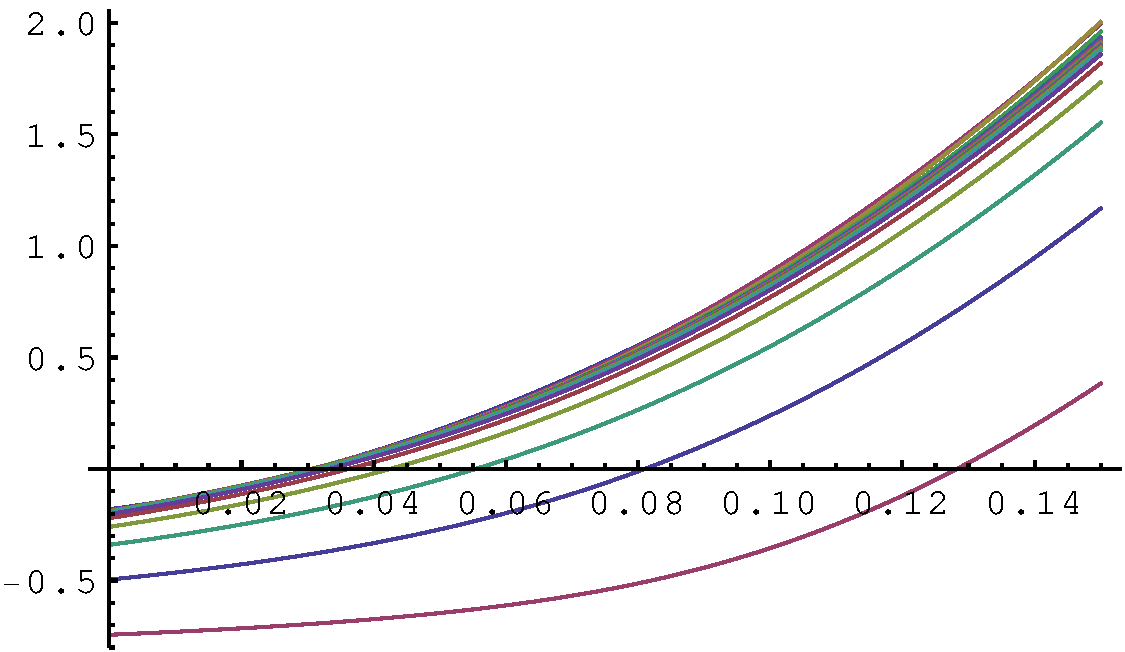
\includegraphics[scale=0.65]{img/chap4/u_flow_ising.pdf}
\caption{The potential for the Ising model at different times (local potential approximation was used). The accumulation of shapes tells us that we started close from a fixed point.}
\label{fig:u_flow_ising}
\end{center}
\end{figure}

An idea is to start from an initial shape for the potential, plug it in the flow equation to see how the potential evolve in time. If at first the potential is almost stationary, that means we have started close from a critical point. By trial and error, we can start closer and closer from the critical point. Once we have a sufficient precision, we can computing the critical exponents associated to this critical point. I tried this method with some success on the Ising model (fig. \ref{fig:u_flow_ising}).
Several drawbacks entail this method. First, we have to solve a partial differential equation, which take some time. Secondly and more importantly, once we have found a critical point, it is hard to know which one it is if there exist several ones (which is the case for the Lifshitz model in $d = 3$).

For all this reasons, I used another approach: solving directly the fixed point equation, which is only a differential equation. This approach has, as we are going to see, the extra advantage of letting one locate with ease a fixed point of interest.

\subsection{Method}
The equation we are interested in solving is 
\begin{equation}
0 = -d_m u(\rho) +(\theta \eta_\sslash + d_m - 4 \theta) \rho u'(\rho) + 8 v_m v_{d-m} \left( l_0^{dm}\left(u'(\rho) + 2 \rho u''(\rho) \right) + (n-1)l_0^{dm}\left(u'(\rho)\right) \right)
\end{equation}
Recalling that the $l_0$ functions are defined by an integral, we see that this is a nonlinear differential algebraic equation, whose general solution is not known. One may wonder if there exists a clever choice of regulator that let us compute the integral, thus turning the nonlinear differential algebraic equation into a simple nonlinear differential equation. 
For the Ising model (in the local potential approximation), such a form of regulator is indeed known\footnote{It is the so-called $\theta$ regulator, $R_t(q)= (k^2-q^2) \theta\left(1-q^2/k^2\right)$}. For the Lifshitz model, it is not known if there exists a regulator allowing one to compute the integral explicitly. However I found a form of regulator allowing one to compute the integral approximately. Under this approximation - which we will explicit and justify later - the fixed point equation becomes
\begin{equation}
\label{eq:u_approx}
0 = u(\rho) - a(\theta, \eta)  \rho u'(\rho) + b_1(\theta, \eta) b_2(\theta, \eta, \rho_0) \left( \frac{1}{1 + \rho_0 + u'(\rho) + 2 \rho u''(\rho)} + \frac{n-1}{1+\rho_0+u'(\rho)} \right)
\end{equation}
This is a second order non-linear differential equation that depends on three parameters: $\eta$, $\theta$ and $\rho_0$.

\begin{figure}[htp]
\centering
\begin{subfigure}{.33\textwidth}
	\centering
	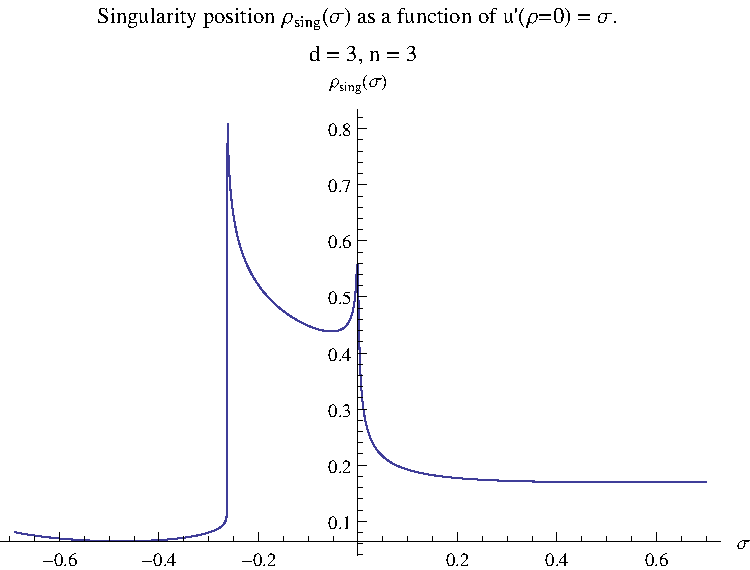
\includegraphics[width=.9\linewidth]{img/chap4/on_d3_n3.pdf}
	\caption{}
	\label{on_d_3}
	\end{subfigure}%
\begin{subfigure}{.33\textwidth}
	\centering
	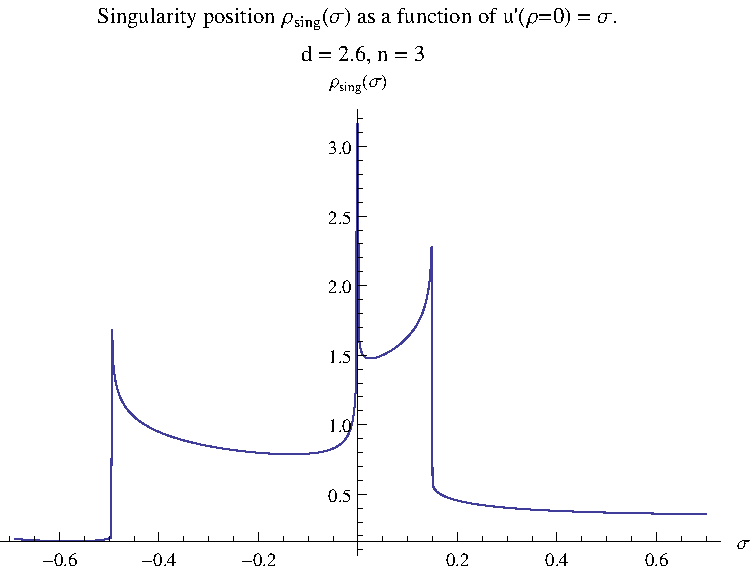
\includegraphics[width=.9\linewidth]{img/chap4/on_d2p6_n3.pdf}
	\caption{}
	\label{on_d_2p6}
\end{subfigure}%
\begin{subfigure}{.33\textwidth}
	\centering
	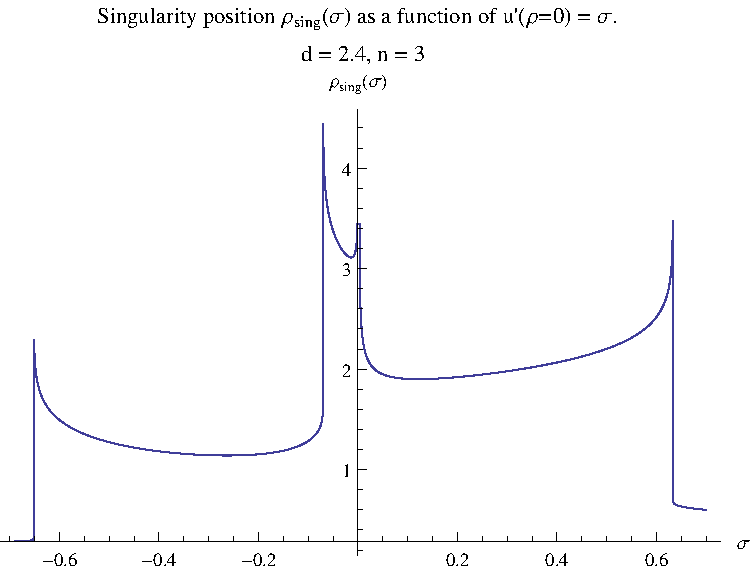
\includegraphics[width=.9\linewidth]{img/chap4/on_d2p4_n3.pdf}
	\caption{}
	\label{on_d_2p4}
\end{subfigure}
\caption{Plot of the (numerically computed) explosion time for the $O(n)$ model in the local potential approximation. We see that in $d=3$ only two physical solutions exist. They are the Gaussian fixed point, at $\sigma = 0$, and the Wilson-Fisher fixed point at its left. A second fixed point appears at $d = 5/7 \simeq 2.6$, and a third one at $d= $.}
\label{fig:on_fp}
\end{figure}

We let  define $\sigma \define u'(0)$. Then, assuming that $u''(\rho)$ is regular around $\rho = 0$ (which is always the case for a physical solution), we have $u(0) = n b_1 b_2/(1+\sigma)$. The knowledge of $u(0)$ and $u'(0)$ uniquely define a solution $u_\sigma(\rho)$.
Now, because of the nonlinearities of the differential equation, we expect most solutions to exhibit a ``finite time blow-up'' behavior, \textit{ie} we expect the $u_\sigma$ or one of its derivative to diverge at some finite ``time'' $\rho = \rho_\sigma^d$.
This is indeed what happens for all values of $\sigma$ except a finite number of them. We must not forget that $u$ is the physical potential. There are no reasons it should not be defined for all values of the field. Therefore the set of physical solutions must included in the (finite) set of solutions defined for all values of the field\footnote{Actually, it turns out that every solution defined for all values of the field is a physical solution. See for example  \cite{CodelloIsing} (Ising model), and \cite{CodelloOn} ($O(n)$ model).}. 
Hunting for critical points is thus extremely easy with this method. Before applying it to the Lifshitz model, we tried the method with the $O(n)$, whose critical points structure is well known. The results are in perfect agreement with our expectations, see fig. \ref{fig:on_fp}. 

For the Lifshitz model, things are a bit more complicated as the equation has three parameters: $\theta$, $\eta_\sslash$ and $\rho_0$. In the local potential approximation, which we have considered here, the first two parameters are taken to their mean field value: $\theta \simeq \theta_{\text{mean field}} =  1/2$, $\eta_\sslash \simeq \eta_{\sslash\text{~mean field}} = 0$. Only one parameter, $\rho_0$, remain.
We recall that this parameter is driving the Lifshitz transition (it is the horizontal axis of the phase diagram \ref{fig:phase_diagram}). Therefore the physics of the Lifshitz model is essentially encoded in the value of this parameter, and we surely cannot approximate it by its mean field value $\rho_{0\text{~mean field}} = 0$.

We have adopted the following strategy:
\begin{itemize}
\item Start at $d=d_c^>$, where mean field is exact in the sense that $\rho_0 = 0$.
\item Slightly decrease the dimension: $d \rightarrow d - \delta d$. 
\item Find the how the Lifshitz point has been displaced and the value of $\rho_0$ modified by this shift in dimension.
\item Go back to step two.
\end{itemize}
We follow this algorithm until we reach $d=3$, at which point our results concerning critical exponents can be compared with the one obtained from other works.

\subsection{Fixed point potential at the Lifshitz critical point}

\begin{figure}[htp]
\begin{center}
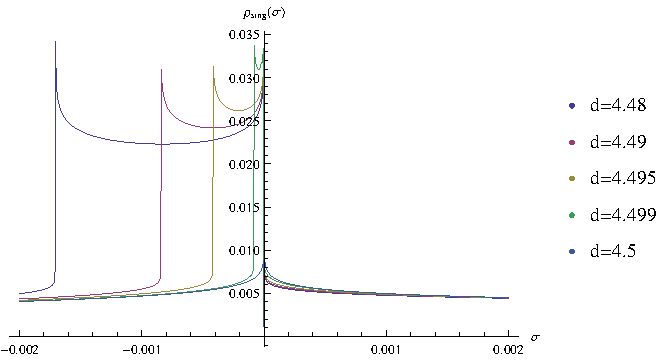
\includegraphics[scale=1]{img/chap4/emergence_lif.pdf}
\caption{Emergence of the Lifshitz fixed point (at the left of the $\sigma = 0$ Gaussian fixed point), when $d$ is slightly lowered, starting from $d_c^>$. Here we have chosen $m=1$ (and thus $d_c^> = 4.5$) and $n=3$.}
\label{fig:emergence_lif}
\end{center}
\end{figure}

As we have seen, the fixed point equation of the Lifshitz model depend on an extra parameter $\rho_0$, contrary to the fixed point equation of the $O(n)$ model. Because this parameter varies locally, a global picture of the explosion time such as the one shown in fig.  \ref{fig:on_fp} does not exist for the Lifshitz model. However close to the upper critical dimension, it is possible to make a local picture of the emergence of the Lifshitz fixed point (fig. \ref{fig:emergence_lif}).

\begin{figure}[htp]
\centering
\begin{subfigure}{.5\textwidth}
	\centering
	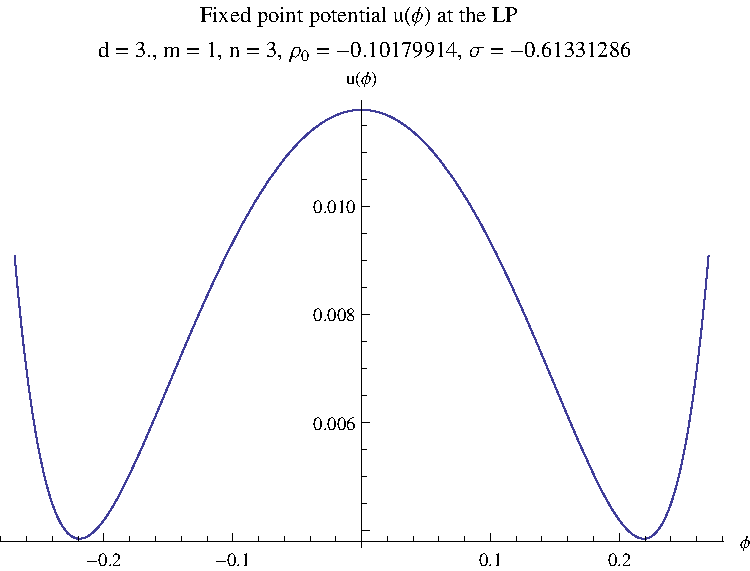
\includegraphics[width=.9\linewidth]{img/chap4/plotfieldd3.pdf}
	\caption{}
	\label{fig:plotfield}
	\end{subfigure}%
\begin{subfigure}{.5\textwidth}
	\centering
	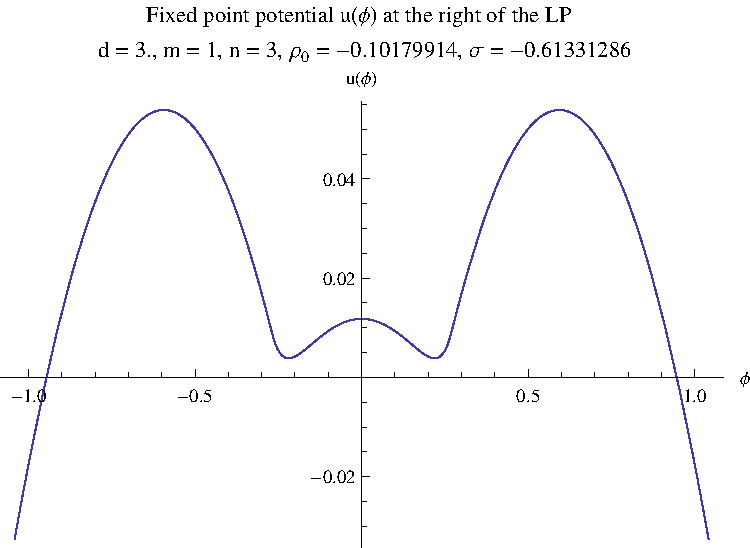
\includegraphics[width=.9\linewidth]{img/chap4/plotfieldrightd3.pdf}
	\caption{}
	\label{fig:plotfieldright}
\end{subfigure}
\caption{Shape of the potential at the Lifshitz point (left image) and and close to it (right image). $\phi$ is the module of the field (here tridimensional): $\phi \define = \sqrt{\phi_i \phi_i}$.}
\label{fig:pot_d3}
\end{figure}

Figure \ref{fig:plotfield} shows the shape of the dimensionless potential at the Lifshitz point. It has the standard ``Mexican-hat'' structure. Note that for an initial condition $\sigma$ very close to the LIfshitz point initial condition, the shape of the potential is completely different (fig. \ref{fig:plotfieldright}). In particular it has the unphysical properties of going to $-\inf$ in the large field limit, meaning that it is not a confining potential. This high sensitivity to the variations of $\sigma$ in the neighborhood of the Lifshitz (in fact any) fixed point allowed us to fine-tune the value of $\sigma_{\text{Lifshitz}}$ up to 12 decimal places very easily. This fine-tuning is essential in order to obtain accurate critical exponents.

\begin{figure}[htp]
\begin{center}
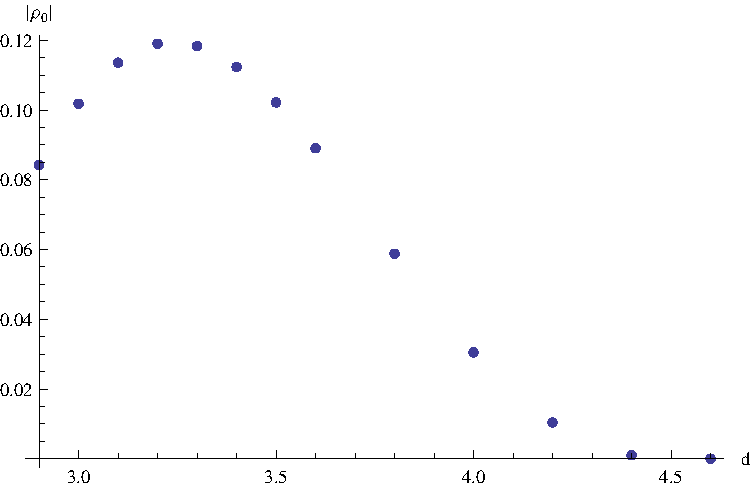
\includegraphics[scale=1]{img/chap4/rhod.pdf}
\caption{The parameter $\rho_0$ as a function of the space dimension $d$.}
\label{fig:rhod}
\end{center}
\end{figure}

To compute $\rho_0$, we make use of the its flow equation (eq. \ref{eq:flow_rho}). At a fixed point, it simply is an algebraic equation on $\rho_0$, depending parametrically on the fixed point potential, which depends parametrically on $\rho_0$.  This means that formally we can write the problem as the self-consistent equation $\rho = f(\rho, u(\rho))$. To solve the problem we simply compute iteratively the sequence $\rho^{(n+1)} = f(\rho^{(n)}, u(\rho^{(n)}))$ until we reach a fixed point. By starting close to $d_c^>$ and progressively going down in dimension we thus obtain $\rho_0$ at the Lifshitz critical point as a function on $d$. The result is shown in fig. \ref{fig:rhod}. 

In is interesting to note that $\rho_0$ is not monotonically increasing in module as we go down in dimension: it reaches a maximum at $d \simeq 3.2$ and goes down again. This non-monotony could be a precursor at the local potential level (\textit{ie} with the approximation that $\eta_\sslash = \eta_\perp  = 0$) of the non-monotony of the anomalous dimensions. Indeed, as was pointed out in \cite{MouhannaLif}, not only are the anomalous dimensions of the Lifshitz model non-monotonous, but even more interestingly, the anomalous dimension $\eta_\sslash$ vanishes below the upper critical dimension. This very peculiar behavior seemingly inherent to the Lifshitz model  is yet to be understood on physical grounds.

Before we go on with the computation of the critical exponents, we will say a word on the numerical methods we used. For solving the nonlinear differential equation on the potential (eq. \ref{eq:u_approx}), a simple Runge-Kutta method did not prove sufficiently accurate, because of the stiffness of the equation. Two methods were found well adapted to this stiff equation: Burlisch-Stoer's extrapolation scheme and the backward differentiation formula method. The latter proved the most accurate in our case. We therefore ended up using an order 5 BDF method to solve or fixed point equation.\footnote{The BDF implicitly express $u(\rho + \Delta \rho)$ in terms of $u(\rho)$, $u(\rho - \Delta \rho)$, $u(\rho - 2 \Delta \rho)$... At each ``time step'' $\Delta \rho$, this implicit equation must be solved to get $\rho + \Delta \rho$. We used Newton's method for that purpose.} 
To solve the algebraic equation on $\rho_0$ we simply used Newton's method.

\subsection{Critical exponents}

\begin{figure}[htp]
\centering
\begin{subfigure}{1.\textwidth}
	\centering
	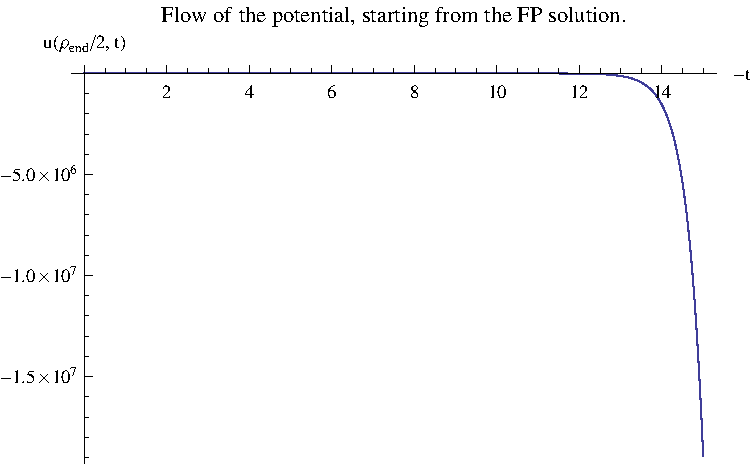
\includegraphics[width=.5\linewidth]{img/chap4/plotflowd3.pdf}
	\caption{Flow of the potential. Numerically, the potential is defined for $\rho \in [0, \rho_{\text{end}}]$ and here we chose arbitrarily to plot it at $\rho = \rho_{\text{end}}/2$.}
	\label{fig:plotflow}
	\end{subfigure}\\
\centering
\begin{subfigure}{.5\textwidth}
	\centering
	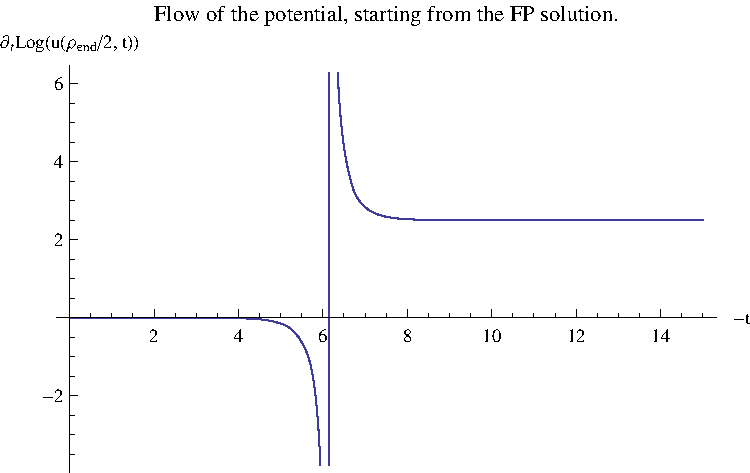
\includegraphics[width=.9\linewidth]{img/chap4/plotlogflowd3.pdf}
	\caption{}
	\label{fig:plotlogflow}
	\end{subfigure}%
\begin{subfigure}{.5\textwidth}
	\centering
	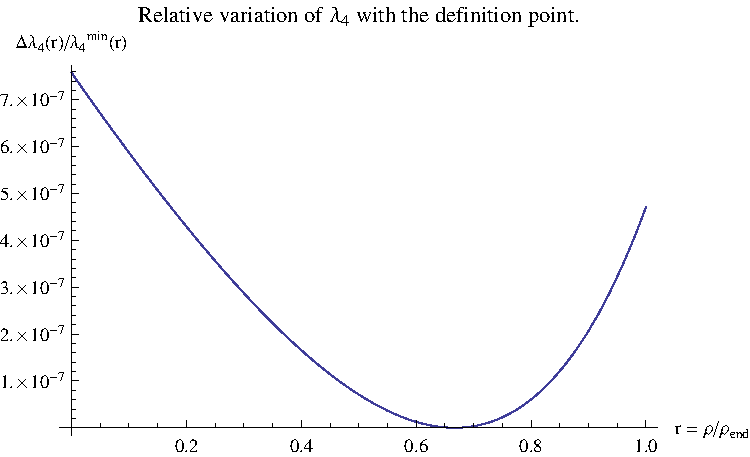
\includegraphics[width=.9\linewidth]{img/chap4/plotnud3.pdf}
	\caption{}
	\label{fig:plotnu}
\end{subfigure}
\caption{}
\label{fig:flow}
\end{figure}

We recall that close to criticality the correlation length behaves as $\xi \propto |T - T_c|^{-\nu}$. 
In the case of the Lifshitz model, the existence of two nonequivalent directions implies the existence of two correlation lengths, and of two critical exponents traditionally denoted $\nu_4$ and $\nu_2$, corresponding to correlation lengths in the $\sslash$ and $\perp$ directions respectively. 

If we had numerically computed the fixed point potential $u(\rho)$ with infinite accuracy, then, when plugging it as an initial condition of the flow equation for the potential (eq. \ref{eq:flow_u}), it should not evolve at all. That is to say, we should have $u_t(\rho) = u(\rho)$ for all $t$. 
Of course, we always have a finite accuracy on the fixed point potential, and when plugging it as an initial condition of the flow equation, the potential evolve in time, slowly going away from the critical surface. In the Lifshitz case two ``directions'' in the space of coupling constants are relevant ; one corresponding to $\nu_4$ and one corresponding to $\nu_2$. We thus have, 
\begin{equation}
u_t(\rho) = u(\rho) + \delta u_4(\rho) e^{\lambda_4 t} + \delta u_2(\rho) e^{\lambda_2 t}
\end{equation}
at the dominant order.
As we have seen, $\nu_4 = 1/\lambda_4$ and $\nu_2 = 1/\lambda_2$. Since $\nu_4 = \theta \nu_2 \leq \nu_2$, we have
\begin{equation}
u_t(\rho) \simeq u(\rho) + \delta u_4(\rho) e^{\lambda_4 t} 
\end{equation}
in the long time limit. That is to say, we should have $\p{t} \log{u_t(\rho)} \simeq \lambda_4$ when $t$ is sufficiently large. This is exactly what we obtain (fig. \ref{fig:plotlogflow}).
This is how we measured $\lambda_4$ and thus $\nu_4$. We found 
\begin{align}
\nu_4 = 0.3999 \\
\nu_2 = 0.7999
\end{align}
We may wonder if these results depend on the point $\rho$ at which we compute $\p{t} \log{u_t(\rho)}$. We computed the relative variation of $\lambda_4$ with respect to the definition point (fig. \ref{fig:plotnu}), to see that these variations only affect the sixth decimal place in the exponent. They are therefore completely negligible compared to other sources of errors.

The values of the critical exponents we found are in very good agreement with the perturbative expansion at order $\epsilon^2$ (see for example \cite{MouhannaLif}).
They also agree well with results obtained with another non-perturbative approach using the so-called Wilson-Polchinski equation (see \cite{BervillierLif}). 


So, apparently, the study conducted during this internship was only successful in finding the same results with a new method!
However, contrary to the Wilson-Polchinski approach, ours can be very easily extended to take into account the anomalous dimensions. In fact, computing the anomalous dimensions is as simple as computing $\rho_0$. All we have to do is use the fixed point (algebraic) equations on $\eta_\sslash$ and $\eta_\perp$ we have already derived, to find the values of the anomalous dimensions, in a fashion completely similar to what have been done concerning $\rho_0$. This has not been done during the internship simply because of a lack of time.

Taking the anomalous dimensions into account completely modifies the values of the critical exponents (cf. \cite{MouhannaLif}). So, they seem to play a crucial role in the physics of the Lifshitz model. 
In that respect, it is interesting to note that continuation of the work began during this internship should provide us with values of the anomalous dimensions, computed with unpreceeding precision.\footnote{The anomalous dimensions have already been computed within the nonperturbative framework, at order 12 in the field. Our method should give us more precise results as it takes into account all orders in the field.}